\chapter*{Introduction}

The journey of Morse theory begins in the $1920$s, when a young Marston Morse, immersed in Poincaré's ``Analysis Situs'', publishes a paper that relates for the first time the critical points of a differentiable function with the topology of the space on which it is defined \cite{BottMarstonMorse}. From then on, numerous mathematicians would put their minds at the service of the development of this theory, giving rise to what we know today as Morse theory. We will not provide an exhaustive list, but there are some whom we will indeed mention: in the first place, John Milnor, who in $1959$ uses Morse theory to prove the existence of the first \textit{exotic sphere} \cite{milnor2010manifolds}; and in the second place, Stephen Smale, who proves the \textit{Poincaré conjecture} true for dimensions greater than four and extends the techniques used to prove the \textit{h-cobordism theorem} \cite{bott1988morse}. % TRANSLATOR: "prueba cierta la conjetura de Poincaré" is garbled in the original; translated by intended meaning.

In $1963$, Milnor takes on the task of compiling in a more modern language the foundations of Morse theory; this work crystallizes in his book ``Morse Theory'' \cite{milnor1963}. In this book he presents a multitude of results within a reduced space, however, this comes at the price of leaving out technical aspects necessary for an inexperienced reader to understand them. In the present work, we seek to present the foundations of Morse theory, from the Morse Lemma (\ref{lemamorse}) to the Morse inequalities (\ref{sec:desigmorse}), in a modern and comprehensive language, and including as much theory as necessary to make it as self-contained as possible. % TRANSLATOR: "comprensivo" in the original is a false friend (Spanish for "sympathetic"); rendered as "comprehensive" per the surrounding sentence.

As we have already mentioned, Morse theory relates the critical points of a differentiable function with topology. The critical points of a function are classified according to whether their Hessian matrix is singular or not at them, being called in the second case \textit{non-degenerate critical points}. Non-degenerate critical points have the particularity that in a neighborhood of theirs there exists a local coordinate system with respect to which the function is expressed as a quadratic form; which implies that they are isolated.

A real-valued function on a smooth manifold whose critical points are all non-degenerate is known as a \textit{Morse function}. By studying the sublevel spaces $M^a=\{q\in M| f(q)\le a\}$ of a Morse function $f:M\to\mathbb{R}$ one can learn how the topology of $M$ changes when passing through the critical points. Theorem \ref{cwvariedad} establishes that if all the sublevel sets are compact, then the homotopy type of the manifold is that of a CW-complex with as many cells of dimension $\lambda$ as critical points of index $\lambda$ $f$ has. Moreover, the Morse inequalities make use only of the number of critical points of each possible index to determine the Euler--Poincaré characteristic and bound the Betti numbers of the manifold.

In essence, Morse theory allows us to know a great amount of information about the topological invariants of a manifold knowing only indices of critical points. Procedures that previously required complex algebraic arguments and techniques are reduced to basic techniques of analysis.

Returning to the results mentioned above, Milnor constructs a manifold equipped with a differentiable structure and proves that it is homeomorphic but not diffeomorphic to the $7$-dimensional sphere $\mathbb{S}^7$. A manifold of this kind is known by the name of exotic sphere, and the way in which he proves that it is homeomorphic to $\mathbb{S}^7$ is by defining on it a Morse function with only two critical points \cite{milnor2010manifolds} (see \ref{reeb}). The case of the h-cobordism theorem is more complicated, but let us say that its proof begins with the definition of a Morse function on the cobordism and, making use of it, gives its decomposition into handles \cite{milnor2025lectures}.

An example with which to illustrate Morse theory is the following. Suppose we have the torus resting on a plane as in Figure \ref{fig:toro}, and we define on it the function $f:T^2\to \mathbb{R}$ that takes each point to its height with respect to the plane.
\begin{figure}[H]
    \centering
    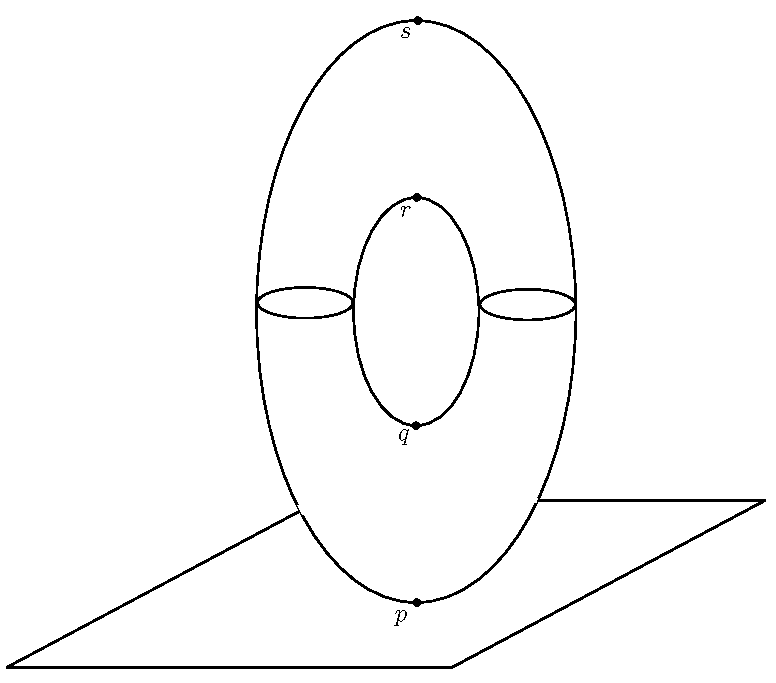
\includegraphics[width=0.5\textwidth]{imagenes/toro_vertical_cropped.pdf}
    \caption{Torus resting on a plane.}
    \label{fig:toro}
\end{figure}

Well, $f$ is a Morse function with four critical points, a minimum ($p$), a maximum ($s$) and two saddle points ($q$ and $r$). Let $a\in\mathbb{R}$, the following holds:
\begin{enumerate}[label=(\roman*), noitemsep]
    \item If $a<f(p)$, $M^a$ is empty.
    \item If $f(p)< a< f(q)$, then $M^a$ is homeomorphic to a $2$-disk.
    \item If $f(q)<a<f(r)$, we have that $M^a$ is homeomorphic to a cylinder.
    \item If $f(r)<a<f(s)$, $M^a$ is homeomorphic to a compact manifold with a circle as boundary.
    \item If $f(s)<a$, $M^a$ is the full torus.
\end{enumerate}
Let us call these regions, in order, $M^{a_0}$, $M^{a_1}$, $M^{a_2}$, $M^{a_3}$ and $M^{a_4}$. In order to describe how the topology of $M^a$ changes as it passes through each critical point, it is necessary to know their indices. The indices of $p$ and $s$ are $0$ and $2$ respectively; the indices of $q$ and $r$ are both $1$.

Now, in terms of homotopy, $M^{a_1}$ is indistinguishable from a point. When passing to $M^{a_2}$, the homotopy type changes to that of a $2$-disk with a $1$-cell attached, the same as that of the cylinder. When we pass to $M^{a_3}$, once again the change in homotopy type corresponds to attaching a $1$-cell. Finally, when we reach $M^{a_4}$, a $2$-cell is attached and one has the homotopy type of a CW-complex with two $2$-cells and two $1$-cells. That is, with this sequence of steps we have recovered the homotopy type of the torus \cite{milnor1963} \cite{bott1988morse}. % TRANSLATOR: "two 2-cells and two 1-cells" reproduced as in the original; the complex described actually has one 0-cell, two 1-cells and one 2-cell (see IDEAS.md).

This result is not particular to the torus in this position, it is general: Morse theory allows us to reproduce this same process for any manifold. We will prove that the topology of the sublevel sets changes only when passing through a critical point. In particular, we will prove that if $M^a$ and $M^b$ are such that there exists no critical point $p\in M$ such that $a<f(p)<b$ and $f^{-1}[a,b]$ is compact, then $M^a$ is a deformation retract of $M^b$ and, in fact, they are diffeomorphic (Theorem \ref{retractodef}). % TRANSLATOR: stray "y" in the original ("$M^a$ y es retracto") dropped.

In the same way, we will prove that if there exists a critical point $p\in M$ satisfying $a<f(p)<b$, then the change in topology is, concretely, the one produced by attaching a $\lambda$-cell to $M^a$, where $\lambda$ is the index of $p$ (Theorem \ref{pegadocelula}).

\iffalse
Among the limitations of Morse theory is the fact that although we can relate the homotopy type of a manifold with that of a CW-complex, it does not tell us how its cells are attached. In the case of the torus, if we only had the Morse function without knowing on which manifold it is defined, we could arrive at the conclusion that it has the homotopy type of a CW-complex with a
\fi
\medskip


In the first chapter we will introduce the notion of non-degenerate critical point and prove the Morse Lemma. In the second chapter we will give a brief formal introduction to CW-complexes and prove the results that describe the procedure used in the example above. The third chapter will be exclusively devoted to developing homology theory, giving constructions of simplicial, cellular and relative homology and presenting the Betti numbers and the Euler--Poincaré characteristic. The fourth and last chapter will be about the Morse inequalities, with a first exposure to certain results on subadditive functions.

